\documentclass[conference]{IEEEtran}
\IEEEoverridecommandlockouts
\pagestyle{plain}
\usepackage{amsmath,amssymb,amsfonts, mathtools}
\usepackage{algorithmic}
\usepackage{graphicx}
\usepackage{subcaption}
\usepackage[hidelinks]{hyperref}
\usepackage{textcomp}
\usepackage{xcolor}
\usepackage[inline]{enumitem}
\usepackage{minted}
\usepackage{tikz}
\usepackage{multicol}
\usetikzlibrary{calc,arrows.meta,positioning,arrows, automata, shapes}
\usepackage[
    backend=biber,
    style=alphabetic,
    citestyle=authoryear
]{biblatex}
\usepackage{csquotes}
\addbibresource{ref.bib}

\def\BibTeX{{\rm B\kern-.05em{\sc i\kern-.025em b}\kern-.08em
    T\kern-.1667em\lower.7ex\hbox{E}\kern-.125emX}}
    

\begin{document}
\title{
    Intrinsic Motivation Research in Reinforcement Learning
}

\author{\IEEEauthorblockN{
    Geert Goemaere
}
\IEEEauthorblockA{
    University of Antwerp \\
    geert.goemaere@student.uantwerpen.be}
}
\maketitle

\begin{abstract}
The field of Reinforcement Learning (RL) has managed to solve very complex tasks like video games or robotic tasks without human help. However, a huge weakness of RL remains when rewards are sparse or hard to get: an agent can only act randomly in hopes of discovering something rewarding. Researchers strive to generate interesting agents without rewards at all, a field sometimes called \textit{unsupervised RL}. These \textit{curious} agents often use intrinsic rewards to motivate exploration. I studied the theory behind the existing sub-fields and methods of Intrinsic Motivation, identified hindsight experience replay as branch of further research and explored ideas to improve learning with hindsight experience. I provided experiments in a gridworld setting and a robotic control setting to support my ideas. Based on those results, I propose possible areas of scientific research.
\end{abstract}

\section{Introduction}

In Reinforcement Learning (RL), an \textit{agent} gathers \textit{rewards} from an \textit{environment} while performing a task in that environment. The agent maximizes rewards by learning the optimal sequence of \textit{actions} while performing the task.

The reward may be a score when the agent learns to solve a game, or a distance function when the agent learns to reach a goal. In that case, the reward function is considered \textit{extrinsic}, i.e. provided by the environment specifically for the task. The agent learns by getting extrinsic rewards from the environment. Spectacular results have been obtained using extrinsic rewards on Atari game [\cite{bellemare2013arcade}] with Deep Q-network (DQN) [\cite{mnih2015human}] using deep reinforcement learning (DRL). 

When rewards are scattered or sparse in the environment, approaches relying on obtaining rewards from the environment are most of the time unsuccessful, as agent is not able to learn optimal actions for the targeted task. In addition, behaviour learned by an agent in one environment is hardly reusable in other environments whether it be for the same task or for other tasks. It is difficult for an agent to abstract or generalize decisions in an environment. Such abstract decisions could be: Take the key and go to the door. Those abstract decisions are performed by low-level actions moving in a certain direction, or picking-up an object by a robot controlling different joints. Those abstract decisions are often called \textit{options} [\cite{sutton1999between}]. To perform a certain task, agents often have to learn a set of tasks in a specific order. E.g. a robot grasping and object and putting it into a box should first learn how to grasp an object before it can learn how to put it into a box. There are potentially infinite number of those options in the real-world or a simulator (e.g. robotic tasks). This is an exploration problem in the option space rather than in the state space.

A limitation of deep reinforcement learning algorithms is their inability to learn a shared state representation independently from extrinsic rewards. Nevertheless, an agent could learn on other interesting features than the ground state space alone, allowing DRL algorithms to considerably speed up the learning process [\cite{raffin2019decoupling}].

Alternatively, unlike RL based on extrinsic rewards, developmental learning is based on the trend that babies, and in extension organisms, spontaneously explore the environment and acquire new skills. This is commonly called \textit{intrinsic motivation} (IM), which can be derived from an intrinsic reward. Intrinsic motivation allows learning new skills making the learning process of new tasks easier.

In this research project, I studied the theory behind intrinsic motivation in reinforcement learning by first understanding the lay of the land as provided by a survey on the role of intrinsic motivation in DRL. [\cite{aubret2019survey}]. As the research area is vast, I focus specifically on the skill learning branch, where \textit{hindsight experience replay} (HER) [\cite{andrychowicz2017hindsight}] as intrinsic motivation method will get most focus.

I believe the contribution of my work to to be
\begin{itemize}
    \item providing an overview on the landscape of intrinsic motivation in DRL
    \item charting the benefits of hindsight experience replay (HER) in DRL
    \item studying possible improvements on HER in tabular and deep settings
    \item proposing potential research areas to improve HER + DRL
\end{itemize}{}

In Section \ref{sec:literature_study}, I present related work, along with intrinsic motivation techniques and other approaches to learn from multiple signals. In Section \ref{sec:experiments}, I provide experiments in a tabular setting and deep setting to validate existing and proposed techniques. In Section \ref{sec:conclusion}, I discuss conclusions drawn from experiments. Finally, in Section \ref{sec:future_work}, I propose potential future work to explore and improve Intrinsic Motivation in Reinforcement Learning.

\section{Literature study} \label{sec:literature_study}

\subsection{A survey on intrinsic motivation in reinforcement learning}

This paper [\cite{aubret2019survey}] is a non-exhaustive review of current ongoing research directions, their limitations and their potential perspectives. The overall literature on IM is huge [\cite{barto2013intrinsic}] and the review only considers its application to DRL. It highlights how IM can improve over state-of-the-art DRL algorithms, scaling to large state and action dimension spaces.

Intrinsic Motivation addresses a number of challenges of standard RL:
\begin{itemize}
    \item Sparse rewards; The agent never receives rewards from the environment.
    \item State representation: The agent cannot learn a representation of its observations with independent features.
    \item Building option: The agent is unable to learn high-level decisions independent of the task.
    \item Learning curriculum: The agent can hardly learn a curriculum of subsequent tasks without expert knowledge.
\end{itemize}

IM offers a greater learning flexibility, through the use of a more general reward function, allowing to tackle the challenges raised above when only an extrinsic reward is used.

The RL framework can be reformulated, as done by [\cite{singh2010intrinsically}] and [\cite{barto2004intrinsically}], to incorporate IM. A distinction is made between a primary reward and a secondary reward signals. The primary reward signal is the standard extrinsic reward returned by the environment. The secondary signal is a local reward computed by the agent and thus internal or intrinsic to that agent. This new RL model can be seen in  Fig. \ref{fig:new_rl_model}.
\begin{figure}[h]
\centering
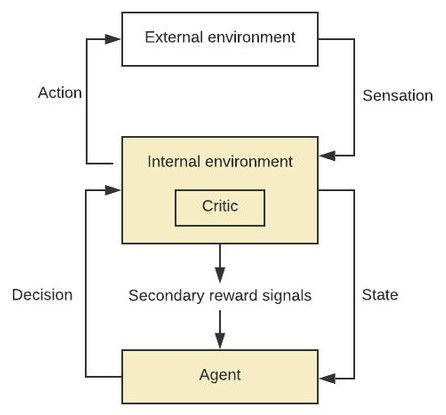
\includegraphics[width=0.9\columnwidth]{img/New-model-of-RL-integrating-IM-adapted-from-Singh-et-al-2010_W640.jpg}
\caption{New model of RL integrating IM, adapted from \cite{singh2010intrinsically}.}
\label{fig:new_rl_model}
\end{figure}

There are multiple ways to integrate an intrinsic reward into a RL framework. The main approach is to compute the agent’s reward r as a weighted sum
of an intrinsic reward $r_{int}$ and the extrinsic reward $r_{ext}$ [\cite{burda2018exploration}; \cite{gregor2016variational};\cite{vezhnevets2017feudal};\cite{huang2019learning}]:
\begin{equation*}
r = \alpha \cdot r_{int} + \beta \cdot r_{ext}
\end{equation*}

This paper [\cite{aubret2019survey} proposes a Classification of the use of IM in RL that emphasizes on two major kinds of IM in RL. This is summarized in Table \ref{tab:classification}.
\begin{table}[h]
  \centering
  \begin{subtable}[t]{0.45\columnwidth}
    \centering
    \begin{tabular}{|p{0.90\textwidth}|}
      \hline
      \multicolumn{1}{|c|}{\textbf{Knowledge acquisition}} \\
      \hline
      \hline
      \textbf{Exploration} \\
      \hline
      Prediction error \\
      State novelty \\
      Novelty as discrepancy towards other states \\
      Information gain \\
      \hline
      \hline
      \textbf{Empowerment} \\
      \hline
      \hline
      \textbf{Learning a relevant state representation} \\
      \hline
      State space as a measure of distance \\
      One feature for one object of interaction \\
      \hline
    \end{tabular}
  \end{subtable}
  \hspace{0em}
  \begin{subtable}[t]{0.45\columnwidth}
    \centering
    \begin{tabular}{|p{0.90\textwidth}|}
      \hline
      \multicolumn{1}{|c|}{\textbf{Skill learning}} \\
      \hline
      \hline
      \textbf{Skill abstraction} \\
      \hline
      Building the goal space from the state space \\
      Mutual information between goals and trajectories \\
      \hline
      \hline
      \textbf{Curriculum learning} \\
      \hline
      Goal sampling \\
      Multi-armed bandit \\
      Adversarial training \\
      \hline
    \end{tabular}
  \end{subtable}
  \caption{Classification of the use of IM in DRL.}
  \label{tab:classification}
\end{table}
\begin{description}
\item[Knowledge acquisition] : The agent strives to find new knowledge about its environment. Knowledge acquisition can improve exploration in sparse reward environments by computing intrinsic reward e.g. based on novelty of states or information gain. It can push the agent to maximize empowerment by rewarding the agent if it is heading towards areas where it controls the environment. It can also help the agent to learn a relevant state representation.
\item[Skill learning] : The agent's ability to construct task-independent and reusable skills in an efficient way. On the one hand it is about the agent's ability to learn a representation of diverse skills in order to achieve them. On the other hand it is about wisely choosing the skills to learn with a curriculum.
\end{description}
The large majority of research in the field is focused on knowledge acquisition. However, my interest is focused on skill learning and this will be the focus of the rest of my research project.
\subsection{Hindsight Experience Replay}
\subsection{The Option-Critic Architecture}
\subsection{Learning Multi-Level Hierarchies with Hindsight}
\section{Experiments} \label{sec:experiments}
\subsection{Tabular Q-Learning}
\subsubsection{Tabular Q-Learning with Hindsight}
\subsubsection{Option Learning with Hindsight}
\subsection{Deep Learning}
\subsubsection{From tabular to deep learning for motor control task}
\section{Conclusion} \label{sec:conclusion}
\section{Future work} \label{sec:future_work}
\newpage
\printbibliography
\end{document}